\section{Analysis \todo{Rephrase}}
\label{sec:analysis}
The Regulus tree depicts the hierarchical structure. We use the color to encode the value of a selected attribute in each node. 
 
\subsection{Attributes}
Each node has several core attributed such as the number of samples the partition contains or the min and max values of the function within the partition. One can potentially precompute additional attributes, such as the mean value, for each partition and store these values in the partition. One of the challenges of this approach is that precomputing all the attributes for all of the nodes can take a very long time. In addition, the user may not use or visualize all of these attributes during the analysis. Finally, the user may want to define new attributes on the fly, again, without precomputing them for each and every partition. 

Instead of precomputing attributes, we define an attribute by providing a factory function to compute its value for a given node and use a caching to compute the value only once when it is requested first. The function can requests other attributes from the tree. We describe our implementation in \autoref{sec:attr-impl}. \autoref{fig:attr-def} depicts a simple attribute definition.

\begin{lstlisting}[language=Python, float=htb, label=fig:attr-def, caption=Attribute definition]
def span(tree, node):
    return node.parent.data.persistence -
           node.data.persistence
tree.add_attr(span)
\end{lstlisting}


\subsection{Models}
We use linear regression to fit a linear model in each partition. There are many possible regression methods: Least squares, Ridge, Lasso, Elastic Net, Lars, etc. 

In general, other models, such as quadratic, can be use although they are more complex and in some sense defeat the purpose. A linear model for d-dimensional data requires d+1 parameters but a a quadratic models require 2 parameters per dimension (for $x_i$ and $x_i^2$) and well as all pairwise permutations $x_i \times x_j$ for a total of $d^2/2$ parameters.

\subsection{Measures}
\label{sec:measures}

\begin{description}
\item[Basic measures] span, min, max, normalize size

\item[Fitness] fitness of the local model to the local data. Note that this is an abstract operation that in general can be different for different models. Since we specify the model and measure independently the detail implementation can be left to the model. Example: \autoref{fig:fitness}

\item[Parent Fitness] the fitness of the parent model to the current node data. Explain why this is an important  measure.

\item[Child Fitness] the fitness of the current model to the data in the parent. Explain what is the purpose.

\end{description}


% \begin{figure*}[htb]
%     \begin{center}
%      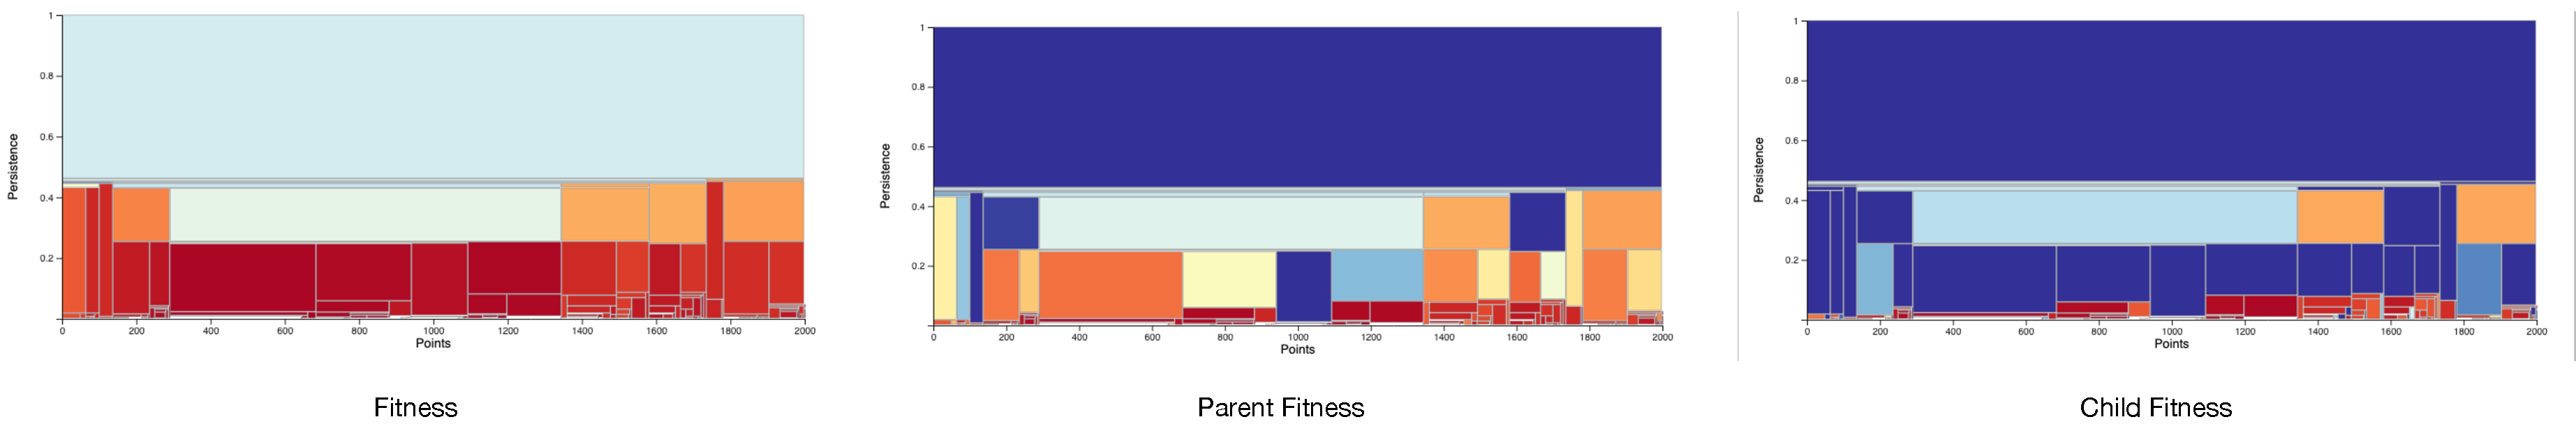
\includegraphics[width=\linewidth]{fitness}
%     \caption{Fitness of: a) local model to local data, b) parent model to local data, c) local model to parent data}
%     \label{fig:fitness}
%     \end{center}
% \end{figure*}
\subsubsection*{Example}
Consider ~\autoref{fig:details}
\begin{itemize}
    \item Root partition (id=0) has lowest fitness. 
    \item Partition 45 (bottom) represent the shallow hill (top left in the 3d view) which does not have a good linear model.
    \item Both partitions 21 and 34 have good linear models (0.944, 0.96) but their models are very different. 
    \item The parent partition (20) has a fitness of 0.770
    \item The Parent Fitness view (bottom right) demonstrates that the model for P0 moderately fit P21 (0.788) and P34 (0.651)
    \item The Child Fitness view (middle right) demonstrates that the models for P21 and P34 don't fit their parent P20 (0.224, -1.866) at all  
 \end{itemize}

% \begin{figure}[htb]
%     \begin{center}
%      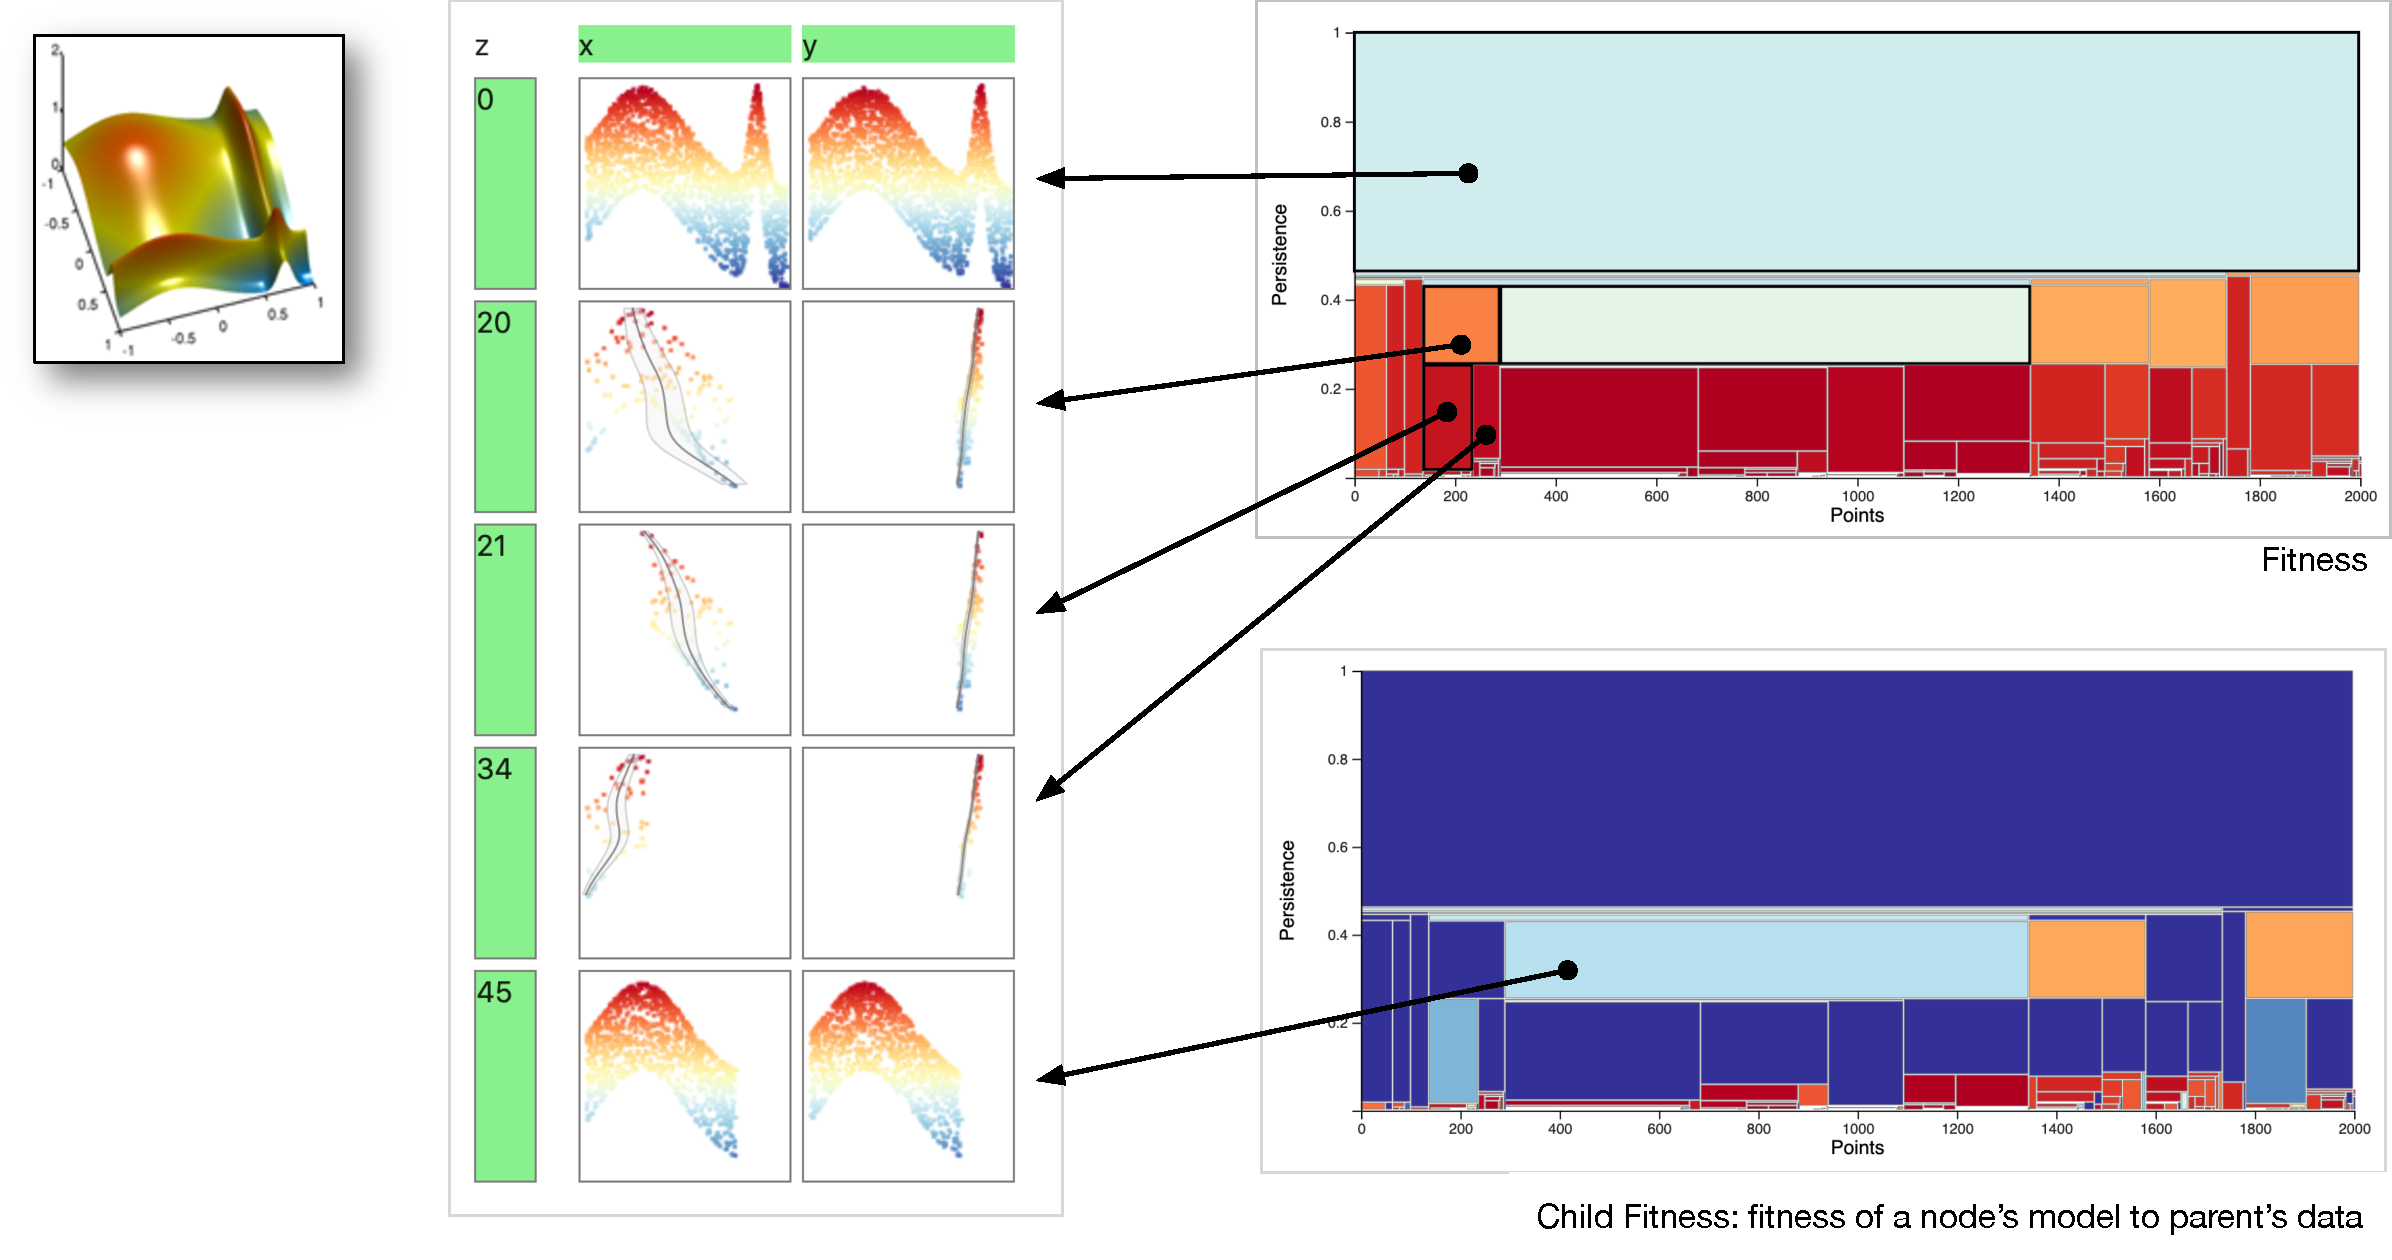
\includegraphics[width=\linewidth]{details}
%     \caption{Partitions Details: left A 3d view of the data. Middle: details view showing projected points for selected partitions. Right: A Regulus Tree where each nodes is colored based on the fitness of the local linear model to the data (red = 1, blue = 0)}
%     \label{fig:details}
%     \end{center}
% \end{figure}

\begin{figure}[thb]
    \begin{center}
     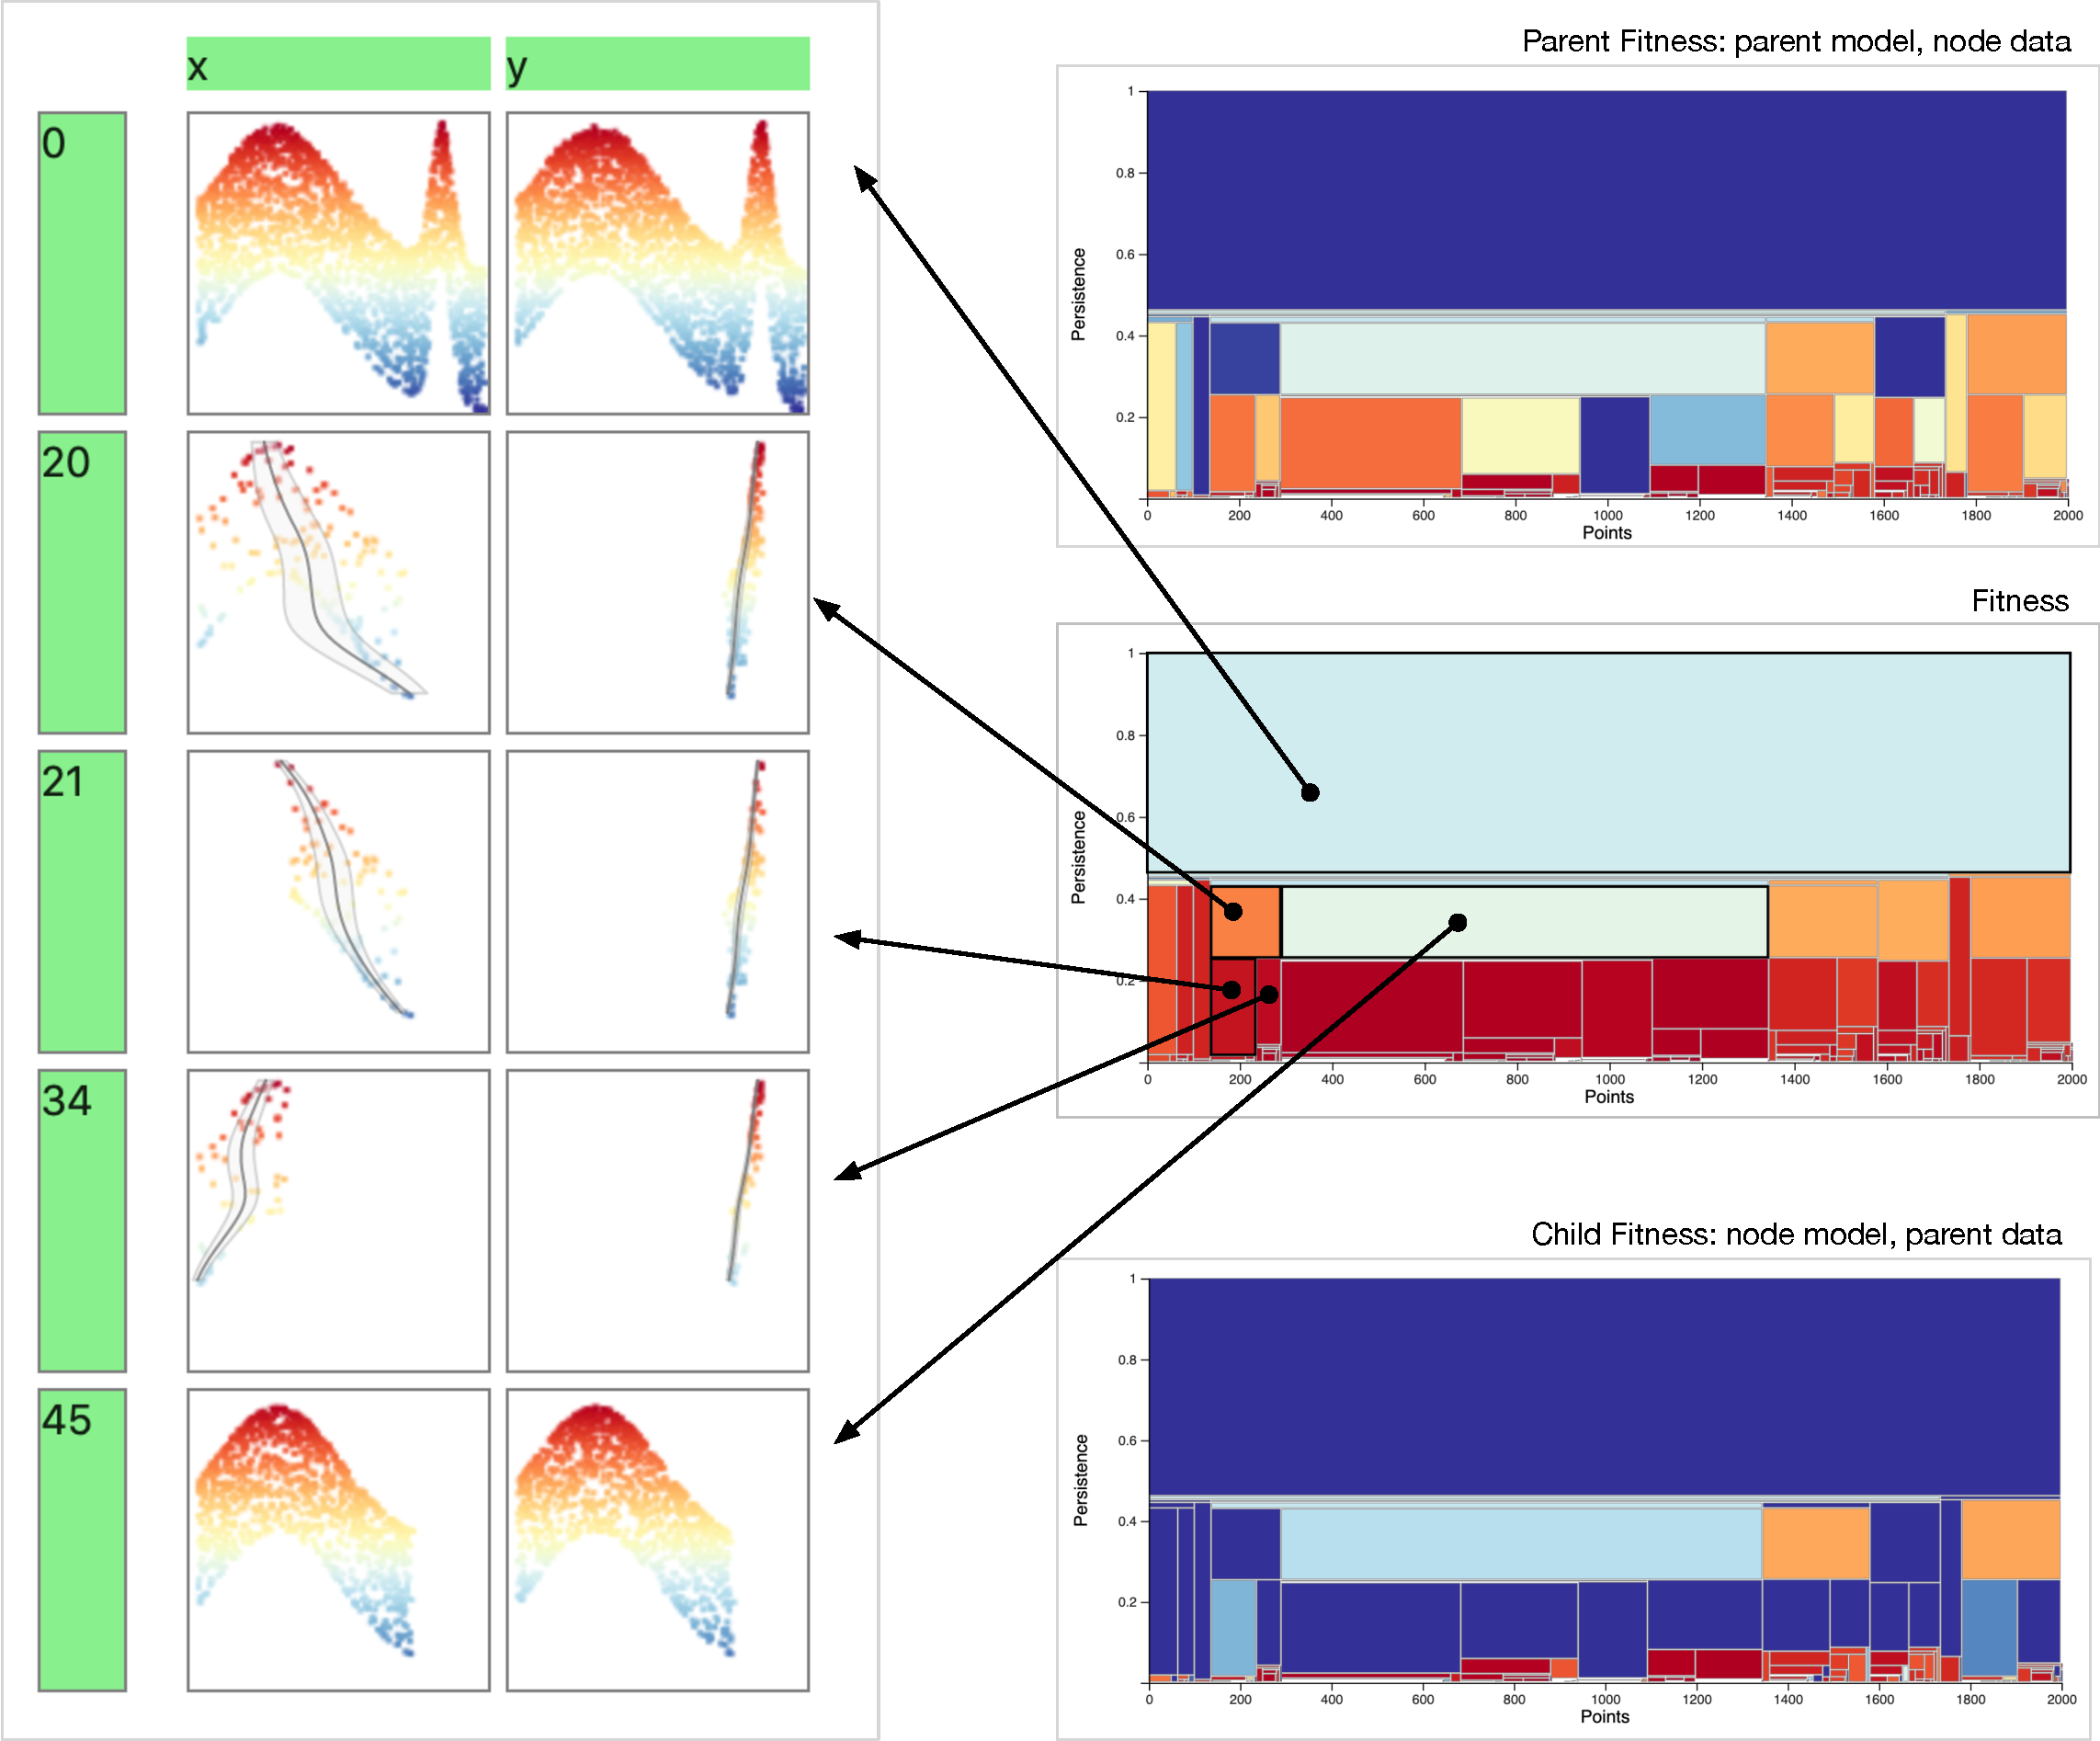
\includegraphics[width=\linewidth]{details-3}
    \caption{Left: details view showing points in selected partitions. Right: Three views of the Regulus Tree, each showing separate fitness measure (red = 1, blue = 0)}
    \label{fig:details}
    \end{center}
\end{figure}

\subsection{Inverse Regression Curves}
\label{sec:inverse-curves}

\begin{itemize}
    \item \textit{"Principal curves are smooth one-dimensional curves that pass through the middle of a p-dimensional dataset, providing a nonlinear summary of the data.They are non-parametric, and their shape is suggested by the data"}~\cite{Tibshirani92}
    \item Gerber~\cite{Gerber10} employed inverse regression curves based on locally weighted regression (LOWESS)~\cite{Cleveland88}. He used the mean std to define a hyper tube around the inverse curve (hyper circle with radium = mean std).
\end{itemize}

Gerber used the inverse regression curves to provide a geometric summary of a partition. For a given persistence level, Gerber displayed the inverse curves after projecting them to a 3D using PCA. This presentation often lead to confusion by users as they tried to assign meaning to the shape of the curves in 3D, which Gerber already noted shouldn't be done.

Describe LOWESSS.

We use the inverse regression curves in two ways. 
\begin{itemize}
    \item show in details view along with $\pm \sigma$, similar to Gerber
    \item use as a skeleton approximation of a partition and use it as a guide to select addition samples
\end{itemize}

\subsection{Sampling}
Choosing samples (partition, n, scale): 
\begin{enumerate}
    \item compute the inverse curve, I, and std deviation for the partition. The curve is computed at n points along the $y_{min} .. y_{max}$ attained in the given partition
    \item compute a hyper tube along the curve with hyper-rectangle cross section $\pm s \times sigma_i$ each dimension, where s is a scale given by the user 
    \item For each of control points of the curve along y, compute the area of the cross section. Normalize by the are of the tube this defines a pdf.
    \item select $k$ values of y using the pdf.
    \item for each selected $y^k$ choose $x_i^k \in [I_i - s \times \sigma, I_i + s \times \sigma]$ 
\end{enumerate}

We run a simulation for each sample. We can use the new data in two ways. First, we can compare each proposed sample with the computed one to evaluate how well our model prediction works. In this case we can add the computed sample to the partition but not reevaluate the MSC. Second, we can restart the whole process and evaluate a new MSC and Regulus decomposition. Note that in this case, the MSC will not necessarily be the same. This is a known issue with MSC and is beyond the scope of this work. 

\begin{figure}[thb]
    \begin{center}
     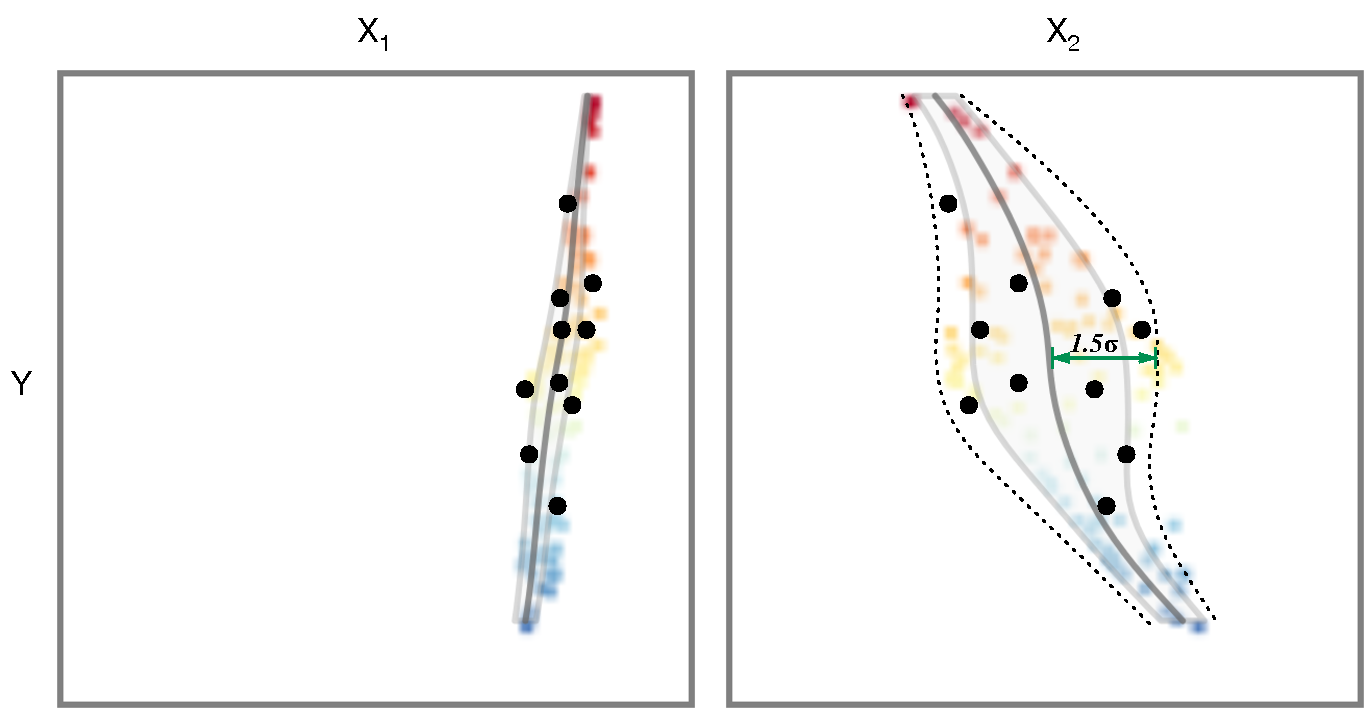
\includegraphics[width=\linewidth]{samples}
    \caption{Selecting samples using the inverse regression curves. The inverse curve is represented by the central gray curve. The two light gray curves represent the area one $\sigma$ around the curve and the dash lines shows the sampling area defined by $s \times \sigma$ where $s$ is a scale given by the user.}
    \label{fig:samples}
    \end{center}
\end{figure}

\subsection{Tree Visibility and Simplification}

\subsubsection*{Nodes Visibility}
Focus on a subset of partitions without changing the tree structure, i.e. only hide irrelevant nodes. For example, focus only on partition with high model fitness but where the model does not fit the parent data well.

\subsubsection*{Tree Reduction}
Instead of hiding nodes one can remove them from the tree. 
One way it to prune the tree based on some criterion (filter). Alternatively, we can reduce the tree by removing individual nodes from the tree based on a given filter and changing the tree structure.


\begin{figure}[htb]
    \begin{center}
     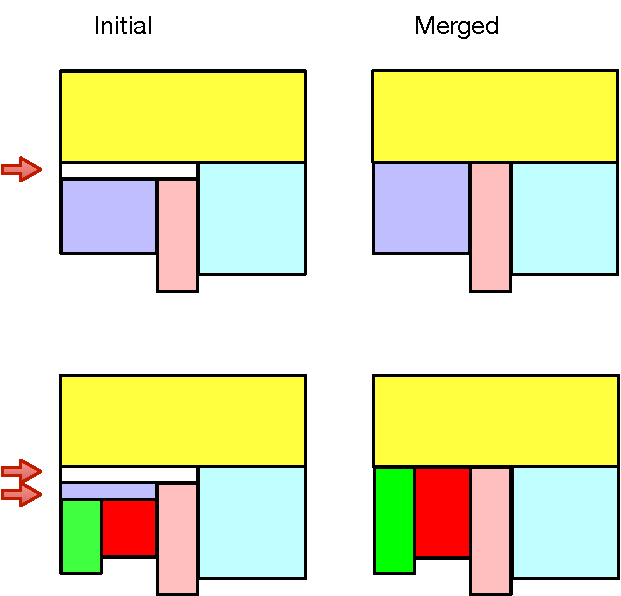
\includegraphics[width=\linewidth]{reduce}
    \caption{Regulus Tree Reduction}
    \label{fig:reduce}
    \end{center}
\end{figure}

\begin{figure}[htb]
    \begin{center}
     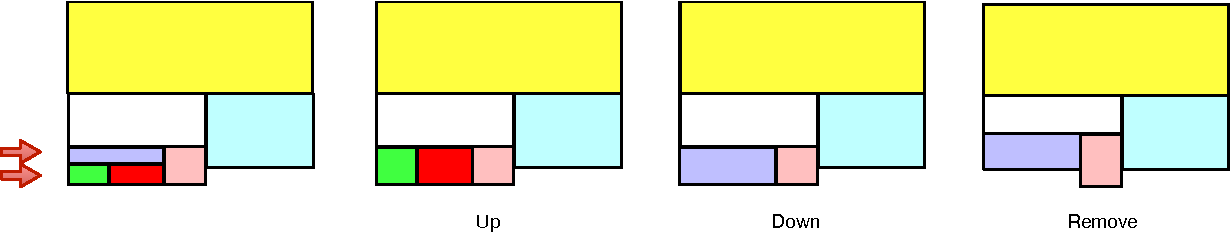
\includegraphics[width=\linewidth]{reduce-leaves}
    \caption{Regulus Tree Reduction at the leaves}
    \label{fig:reduce-leaves}
    \end{center}
\end{figure}